\section{Лекция 7}

\raisebox{.5pt}{\textcircled{\raisebox{-.9pt} {1}}} \underline{задача Дирихле}

\[ {(-\Delta u, u )}_H = \Int_{\Omega} \Sum_{i=1}^{n} {\left(\frac{\partial u }{\partial x_i}\right)}^2 d \Omega \]

При $ n = 2 $
\[ {(-\Delta u, u )}_H = \Int_{\Omega} \left( {\left(\frac{\partial u }{\partial x}\right)}^2 + {\left(\frac{\partial u }{\partial y}\right)}^2 \right) d \Omega \]

\begin{figure}[h!]
	\centering
	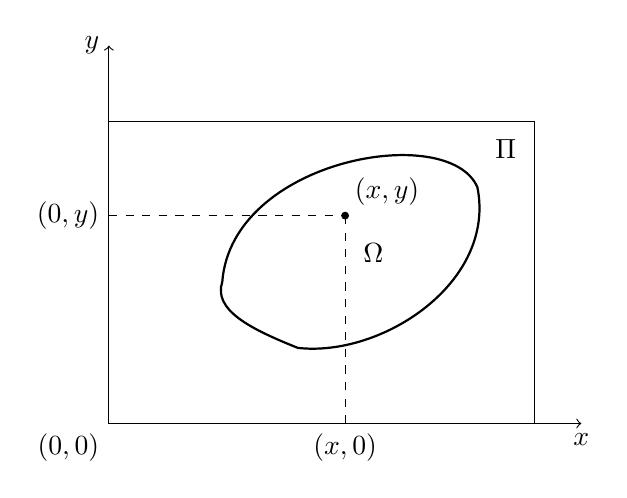
\begin{tikzpicture}[scale=1.2]
		
		% Axes
		\draw[->] (0,0) -- (5,0) node[anchor=north] {$x$};
		\draw[->] (0,0) -- (0,4) node[anchor=east] {$y$};
		
		% Rectangle
		\draw (0,0) rectangle (4.5,3.2);
		\node at (4.2,2.9) {$\Pi$};
		
		% Domain Omega
		\draw[thick] (1.2,1.5) .. controls (1.3,2.8) and (3.6,3.2) .. (3.9,2.5)
		.. controls (4.1,1.5) and (2.9,0.7) .. (2.0,0.8)
		.. controls (1.5,1.0) and (1.1,1.2) .. (1.2,1.5);
		\node at (2.8,1.8) {$\Omega$};
		
		% Point (x,y)
		\draw[dashed] (0,2.2) -- (2.5,2.2);
		\draw[dashed] (2.5,0) -- (2.5,2.2);
		\filldraw (2.5,2.2) circle (1pt) node[anchor=south west] {$(x,y)$};
		
		% Corner points
		\node at (0,0) [anchor=north east] {$(0,0)$};
		\node at (0,2.2) [anchor=east] {$(0,y)$};
		\node at (2.5,0) [anchor=north] {$(x,0)$};
		
	\end{tikzpicture}
	\caption{}
	\label{fig:7.1}
\end{figure}

Заключим $\Omega$ внутрь некоторого прямоугольника $\Pi$ (Рис. \ref{fig:7.1}). Продолжим $u(x, y)$ на весь прямоугольник, полагая ее равной нулю вне $\Omega$
\[ \forall \ A(x_1, y_1) \in \Pi: \]
\[ \Int_{x_{min}}^{x_1} \frac{\partial u(x, y_1)}{\partial x} dx = u(x_1, y_1) - u(x_{min}, y_1) \]
\[ u^2(x_1, y_1) \overset{\text{КБ}}{\leq} (x_1 - x_{min}) \Int_{x_{min}}^{x_1} {\left[ \frac{\partial u(x, y_1)}{\partial x} \right]}^2 dx \leq a \Int_{x_{min}}^{x_{max}} {\left[ \frac{\partial u(x, y_1)}{\partial x} \right]}^2 dx \label{7.1} \tag{7.1} \]

Проинтегрируем это неравенство

\[ \Int_{\Pi} u^2(x_1, y_1) dx_1 dy_1 \leq a^2 \Int_{\Pi} {\left[ \frac{\partial u(x, y_1)}{\partial x} \right]}^2 dx dy_1 \leq \Int_{\Pi} \left( {\left(\frac{\partial u }{\partial x}\right)}^2 + {\left(\frac{\partial u }{\partial y}\right)}^2 \right) d \Omega \]
\[ \Int_{\Pi} u^2(x, y) d\Omega \leq \Int_{\Pi} \left( {\left(\frac{\partial u }{\partial x}\right)}^2 + {\left(\frac{\partial u }{\partial y}\right)}^2 \right) d \Omega \]
\[ {(Au, u)}_H \geq \gamma^2 {\| u \|}_H^2 \]

Получаем, что $A$ положительно определен на $D_A$ \\

Неравенство Фридрихса в общем виде:
\[ \Int_{\Omega}^{} \Sum_{k=1}^{m} \left(\frac{\partial  u}{\partial x_k}\right)^2 d\Omega \geq \gamma^2 \Int_{\Omega}^{} u^2 dx, \qquad u|_S=0 \]

\raisebox{.5pt}{\textcircled{\raisebox{-.9pt} {2}}} \underline{задача Робена}

\[ \left\{ \begin{array}{l}
	- \Delta u = f \qquad \text{в} \ \Omega \\
	{\left. \left[\cfrac{\partial u }{\partial n} + \sigma (P) u (P) \right] \right|}_{\partial \Omega} = 0
\end{array} \right. \]
\[ \sigma(P) \geq \sigma_0 = const > 0 \]
\[ \Int_{\Omega} u^2 d\Omega \leq C \left\{ \Int_{\Omega} \left( {\left(\frac{\partial u }{\partial x}\right)}^2 + {\left(\frac{\partial u }{\partial y}\right)}^2 \right) d\Omega + \Int_{\partial \Omega} u^2 dS \right\} \]
\[ u = f \cdot v \]

\begin{multline*}
	{\left(\frac{\partial(fv)}{\partial x}\right)}^2 + {\left(\frac{\partial(fv)}{\partial y}\right)}^2 = f^2 \left[{\left(\frac{\partial v}{\partial x}\right)}^2 + {\left(\frac{\partial v}{\partial y}\right)}^2\right] - \\ - 
	v^2 f\Delta f + \underbrace{\frac{\partial}{\partial x} \left(v^2 f \frac{\partial f }{\partial x}\right) +  \frac{\partial}{\partial y} \left(v^2 f \frac{\partial f}{\partial y} \right)}_{(*)} \label{7.2} \tag{7.2}
\end{multline*}

Преобразуем правую и левую части:
\begin{multline*}
	{\left( \frac{\partial f}{\partial x} v + \frac{\partial v}{\partial x} f \right)}^2 + {\left( \frac{\partial f}{\partial y} v + \frac{\partial v}{\partial y} f \right)}^2 = v^2 \left( {\left(\frac{\partial f}{\partial x}\right)}^2 + {\left(\frac{\partial f}{\partial y}\right)}^2 \right) + f^2 \left( {\left(\frac{\partial v}{\partial x}\right)}^2 + {\left(\frac{\partial v}{\partial y}\right)}^2 \right) + \\
	+ 2v \frac{\partial v}{\partial x} f \frac{\partial f}{\partial x} + 2v\frac{\partial v }{\partial y} f \frac{\partial f}{\partial y}
\end{multline*}

\[ (*) = 2v \frac{\partial v}{\partial x} f \frac{\partial f}{\partial x} + v^2 \frac{\partial}{\partial x} \left( f \frac{\partial f}{\partial x} \right) + 2v\frac{\partial v }{\partial y} f \frac{\partial f}{\partial y} + v^2 \frac{\partial}{\partial y} \left( f \frac{\partial f}{\partial y} \right) \]

Получим

\[ v^2 \left( {\left(\frac{\partial f}{\partial x}\right)}^2 + {\left(\frac{\partial f}{\partial y}\right)}^2 \right) = - v^2 f \Delta f + v^2 \frac{\partial}{\partial x} \left( f \frac{\partial f}{\partial x} \right) + v^2 \frac{\partial}{\partial y} \left( f \frac{\partial f}{\partial y} \right) \]

что при дальнейшем упрощении очевидно оказывается верным равенством.

Отбрасывая первое слагаемое справа в \eqref{7.2}:
\[
{\left(\frac{\partial(fv)}{\partial x}\right)}^2 + {\left(\frac{\partial(fv)}{\partial y}\right)}^2 \geq - 
v^2 f\Delta f + \frac{\partial}{\partial x} \left(v^2 f \frac{\partial f }{\partial x}\right) +  \frac{\partial}{\partial y} \left(v^2 f \frac{\partial f}{\partial y} \right)
\]

Проинтегрируем получившееся $\Int_{\Omega} (...) d\Omega$

\[ \Int_{\Omega}^{} \left( {\left( \frac{\partial (fv)}{\partial x}\right)}^2 + {\left(\frac{\partial (fv)}{\partial y}\right)}^2 \right) d\Omega \geq - \Int_{\Omega}^{}v^2f\Delta f \, d\Omega + \Int_{\partial \Omega}^{}v^2 f \frac{\partial f}{\partial  n} dS \]
\[ -\Int_{\Omega}^{} vf \Delta f d\Omega \leq \Int_{\Omega} \left( {\left(\frac{\partial u }{\partial x}\right)}^2 + {\left(\frac{\partial u }{\partial y}\right)}^2 \right) d\Omega + \left| \Int_{\partial \Omega}^{} v^2 f \frac{\partial f}{\partial n}d S \right| \]

\[ f = \sin \left(\frac{\pi x}{a}\right) \sin \left(\frac{\pi y }{b}\right) \]
\[ \Delta f = - \pi^2 \left(\frac{1}{a^2} + \frac{1}{b^2}\right) f \]
\[ -\Int_{\Omega}^{}v^2 f \Delta f d\Omega = -\Int_{\Omega}^{} -v^2 f \Delta u^2 (\cdot) d\Omega = \Int_{\Omega}^{} u^2 \pi^2 (\cdot) d\Omega \]
\[ \left| \Int_{\partial \Omega}^{}v^2 f \frac{\partial f}{\partial n} dS \right| \leq \Int_{\partial  \Omega}^{} v^2 f \left| \frac{\partial f}{\partial n} \right| dS \leq c_1 \Int_{\partial \Omega}^{} u^2 dS \]

\[ \pi^2 \left(\frac{1}{a^2} + \frac{1}{b^2}\right) \Int_{\Omega}^{} u^2 d\Omega \leq \Int_{\Omega} \left( {\left(\frac{\partial u }{\partial x}\right)}^2 + {\left(\frac{\partial u }{\partial y}\right)}^2 \right) d\Omega + c_1 \Int_{\partial \Omega}^{} u^2 dS \]
\[ c = \min \left\{ \frac{c_1}{\pi^2 \left( \frac{1}{a^2} + \frac{1}{b^2}\right)}, \frac{1}{\pi^2 \left( \frac{1}{a^2} + \frac{1}{b^2}\right)} \right\} \]

\begin{multline*}
	{(-\Delta u, u)}_H = \Int_{\Omega}^{} (\operatorname{grad} u)^2 d\Omega - \Int_{\partial \Omega}^{}u \frac{\partial u}{\partial n} dS \overset{\eqref{6.6}}{\geq} \Int_{\Omega}^{} (\operatorname{grad} u)^2 d\Omega + \sigma_0 \Int_{\partial  \Omega}^{} u^2 dS \geq \\
	\geq \sigma_1 \left\{ \Int_{\Omega}^{} (\operatorname{grad} u)^2 d\Omega + \Int_{\partial \Omega}^{}u^2 dS \right\}
\end{multline*}
\[ \sigma_1 = \min \{\sigma_0, 1\} \]
\[ \frac{\sigma_1}{c} {\|u\|}_H^2 \leq \Int_{\Omega}^{} (\operatorname{grad} u)^2 d\Omega + \Int_{\partial \Omega}^{}u^2 dS \]
\[ \gamma = \sqrt{\frac{\sigma_1}{c}} \]
\[ -(\Delta u, u)_H \geq \frac{\sigma_1}{c} {\|u\|}_H \]

\newpage